\section{Análisis de Repast for High Performance Computing}

\subsection{Análisis General}

Repast HPC es una herramienta para el desarrollo de simulaciones y
modelados basados en agentes escrito en C++. Está completamente
orientado al procesamiento paralelo, para esto se apoya en alguna
implementación de MPI (``Message Passing Interface'') y un wrapper
provisto por la librería Boost.

Al ser un framework brinda toda la estructura para desarrollar la
simulación y el modelado. De manera resumida, posee las siguientes
características:

\begin{itemize}
	
	\item
	Jerarquía de clases que imitan los objetos de LOGO; Turtles, Patches,
	Links y Observer.
	\item
	Schedulling de eventos, que permite programar eventos periódicos, y
	tener algo similar al paso del tiempo.
	\item
	Contextos, lugar donde residen los agentes.
	\item
	Proyecciones espaciales y lógicas, permiten establecer relaciones
	entre agentes.
	\item
	Comunicación entre procesos, dado las características paralelas del
	framework.
\end{itemize}

Puede utilizarse en cualquier sistema *nix, incluyendo MacOS, Linux y
FreeBSD.

\subsection{Compilación}

Al estar desarrollado en C++, que carece de un gestor de paquetes como
otros lenguajes, las dependencias se tornan problemáticas. Debido a
esto, Repast provee un archivo con las librerías y versiones apropiadas:

https://github.com/Repast/repast.hpc/releases/tag/v2.3.0

Las librerías de las que depende Repast son:

\begin{itemize}
	
	\item
	Herramientas de compilación (g++, make, diff).
	\item
	MPI
	\item
	NetCDF
	\item
	CURL
	\item
	Boost: serialization, system, filesystem y mpi.
\end{itemize}

\subsubsection{Instalación de Dependencias}

La manera más efectiva de instalar todas las dependencias es utilizar el
archivo mencionado anteriormente, siguiendo las instrucciones para la
instalación manual, para el caso de un Linux basado en Debian, los
comandos a ejecutar son los siguientes:

\begin{Shaded}
	\begin{Highlighting}[]
		\BuiltInTok{cd}\NormalTok{ MANUAL\_INSTALL}
		
		\ExtensionTok{apt{-}get}\NormalTok{ update }\KeywordTok{\&\&} \ExtensionTok{apt{-}get}\NormalTok{ install build{-}essential}
		
		\ExtensionTok{./install.sh}\NormalTok{ curl}
		\ExtensionTok{./install.sh}\NormalTok{ mpich }
		\BuiltInTok{export} \VariableTok{PATH=$HOME}\NormalTok{/sfw/MPICH/bin/:}\VariableTok{$PATH}
		\ExtensionTok{./install.sh}\NormalTok{ netcdf}
		\ExtensionTok{./install.sh}\NormalTok{ boost}
		\ExtensionTok{./install.sh}\NormalTok{ rhpc}
	\end{Highlighting}
\end{Shaded}

Todas las librerías y headers son instalados en la carpeta
\texttt{\textasciitilde{}/sfw/}. En la línea 7 se agrega la carpeta de
MPICH a la variable PATH para que Boost y la terminal puedan encontrar
el binario de MPI.

Para ver ejemplos de compilación, puede usarse como guía los ejemplos
que se encuentran en: https://repast.github.io/hpc\_tutorial/TOC.html.

\subsection{Ejecución}

El binario generado debe ejecutarse a través de MPICH (u otra
implementación de MPI), para que se genere el entorno adecuado,
especificando la cantidad de procesos:

\begin{verbatim}
mpirun -n P repast.exe
\end{verbatim}

Siendo P la cantidad de procesos, también puede enviarse parámetros en
caso de que el programa lo requiera.

\subsection{Estructura de un programa de Repast HPC}

Dada la complejidad y el alcance del framework, Repast HPC requiere que
se definan un conjunto de clases para establecer un entorno donde
ejecutar la simulación. Este se compone de la siguiente manera:

\begin{itemize}
	
	\item
	Agentes
	\item
	Programa (\emph{schedule})
	\item
	Contexto
	\item
	Proyección
\end{itemize}

\subsubsection{Agentes}

Implementados como clases de C++, cuyo estado es representado con
variables internas. Y su comportamiento se establece a través de
métodos. Cada agente dispone de un ID único para poder identificarse
dentro de la simulación.

\subsubsection{\texorpdfstring{Programa
		(\emph{schedule})}{Programa (schedule)}}

Como se mencionó, Repast provee un mecanismo para generar eventos
periódicos, basado en \emph{ticks}. Pueden definirse el instante en el
cuál se genera el evento, y su periodicidad.

\subsubsection{Contexto}

Se comporta como un contenedor de toda la población de agentes. Repast
se asegura que no haya dos agentes iguales (mismo ID) en el contexto.

\subsubsection{Proyección}

No es estrictamente necesaria, pero resulta indispensable ya que permite
establecer relaciones entre los agentes. RHPC provee dos tipos de
proyecciones: espaciales y lógicas, la primera se utiliza para modelar
mundos bidimensionales, estableciendo una matriz donde se encuentran
dispuestos los agentes; la segunda permite modelar relaciones genéricas,
a través de grafos, para generar interacción entre agentes.

\subsection{Configuración y Ejecución de la Simulación}

Una simulación de Repast HPC se compone, por lo tanto, de un conjunto de
agentes dentro de un contexto, los cuales poseen un comportamiento
definido a través de métodos. Para realizar estos comportamientos de
manera periódica, se registran en un Scheduler que se encargará de
incremetar los ticks y llamar a los métodos que se hayan específicado
para ese instante de la simulación.

\subsection{Paralelismo}

Repast for High Performance Computing es un framework, como mencionamos,
orientado completamente al cómputo en paralelo. Para esto se apoya en el
protocolo MPI, por lo que se trata de memoria distribuida. Esto afecta
directamente al modelado del problema, ya que cada proceso ejecutando la
simulación posee un conjunto de agentes de los cuales tiene control
total, llamados agentes locales. Para poder relacionarse con el resto de
los agentes de la simulación, que residen en otros procesos, debe
solicitar una copia de los mismos, los cuales pasan a ser denominados
agentes no-locales. Esta comunicación es unidireccional, es decir, los
cambios de estado realizados sobre agentes no-locales no se propagan al
proceso donde se encuentran originalmente. Por este motivo se debe
asegurar que las copias de los agentes en cada proceso estén
sincronizadas con los agentes reales.

De todas formas, es posible mover agentes de un proceso a otro, de
manera de cambiar el proceso que tienen a cargo. Esto resulta útil para
balancear carga y, como analizaremos a continuación, para proyecciones
espaciales.

Por ejemplo, se quiere modelar un juego de tiro al blanco, donde hay dos
agentes, un arquero y un blanco, y donde cada agente se encuentra en
procesos diferentes, A y B. Cuando el arquero dispare una flecha y
acierte en el blanco, el proceso A no puede realizar cambios en el
blanco para reflejar el acierto, ya que este se encuentra en el proceso
B.

\subsubsection{Proyecciones Espaciales}

Para facilitar el paralelismo, Repast HPC provee, para proyecciones
espaciales, una manera de particionar el plano físico. Asignando cada
partición del plano a un proceso diferente, permitiendo dividir la
grilla en M x N procesos.

Ahora los agentes se encuentran distribuidos en diversos procesos, de
acuerdo a su ubicación en el mapa:

\begin{figure}[H]
	\centering
	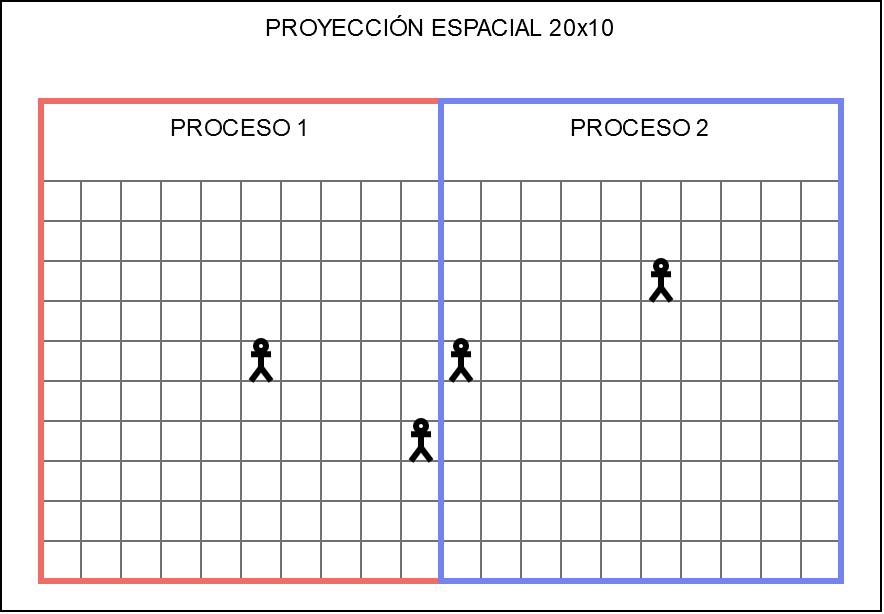
\includegraphics{process_01.png}
	\caption{Partición de una proyección espacial entre 2 procesos}
\end{figure}

Dado que la principal aplicación de una proyección espacial es obtener
otros agentes que se encuentren en la proximidad, surge un problema:
cuando un agente en el \emph{borde} del proceso solicita los agentes que
lo rodean, recibe solo aquellos que se encuentren en el mismo proceso.

Para solucionar esto, Repast agrega una \emph{zona de amortiguamiento}
como seguridad: cuando un agente se acerca al borde es copiado al
proceso adyacente (como un agente no-local, por lo cual no puede
modificarse, pero permite saber de su existencia). De esta manera,
cuando un agente cercano al borde solicite los agentes que lo rodean,
recibirá correctamente los agentes.

\begin{figure}[H]
	\centering
	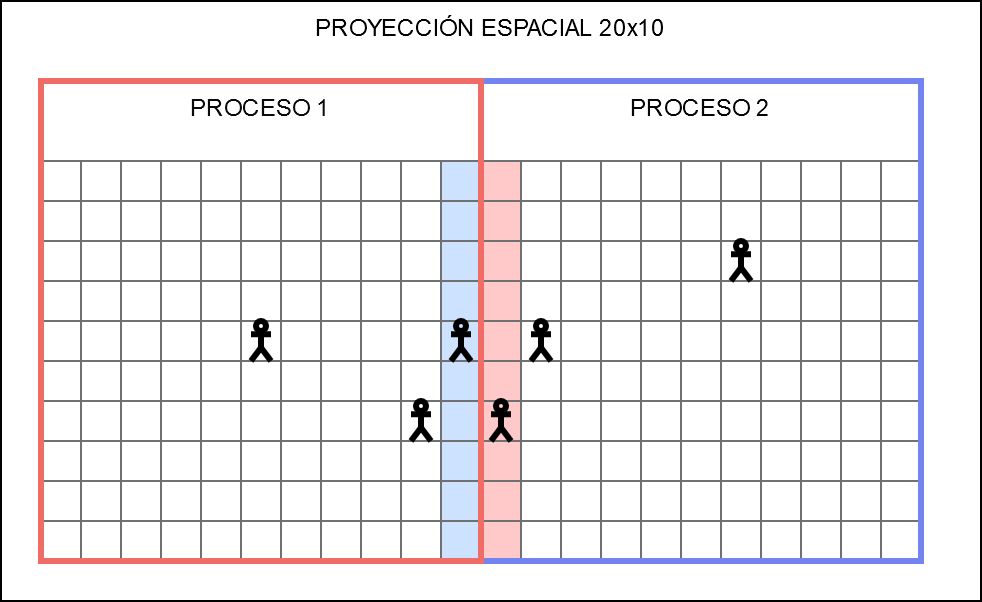
\includegraphics{process_02.png}
	\caption{Partición de una proyección espacial utilizando un colchón para copiar agentes}
\end{figure}

En color puede verse toda la información que fue copiada desde el otro
proceso.

El tamaño de la zona de amortiguamiento es definido por el usuario, una
amortiguación chica reduce la comunicación entre procesos pero reduce la
distancia a la cual ven los agentes en otros procesos. Por lo tanto se
debe establecer el mínimo tamaño posible.
